\documentclass{article}
%\twocolumn
\usepackage{proof}
\usepackage{tikz}
\usetikzlibrary{automata,positioning}
\input{structure.tex} 

\title{Parsly: Procedureless Protocol Compiler\\
		\large A Software Engineering Approach to \\ Simplify Protocol Development Process} 

\author{Han Zheng\\ \texttt{tim.zheng@hivechat.org}} 
\date{ \today} 

\begin{document}
\maketitle 

\section{Introductions} % Unnumbered section


\subsection{The Cycle of Protocol Development}
\begin{figure}[h!]
\begin{center}
\label{fig:developmentCycle}
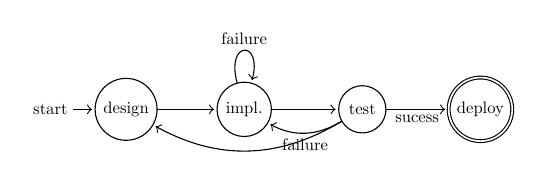
\begin{tikzpicture}[
	shorten >=1pt,
	node distance=2.5cm, 
	on grid, 
	auto, 
	scale=0.6, 
    transform shape, 
    align=center, 
    state/.style={
    	circle, 
    	draw, 
    	minimum size=1cm
    }] 
    
   \node[state,initial] (q_0)   {design}; 
   \node[state, right=of q_0] (q_1) {impl.}; 
   \node[state, right=of q_1] (q_2) {test}; 
   \node[state,accepting, right=of q_2](q_3) {deploy};
   \path[->] 
    (q_0) edge node {} (q_1)
    (q_1) edge node  {} (q_2)
    (q_1) edge [loop above] node {failure} (q_1)
    (q_2) edge node [swap] {sucess} (q_3) 
    (q_2) edge [bend left, below] node {failure} (q_1)
    (q_2) edge [bend left, below] node {} (q_0);
\end{tikzpicture}
\caption{development cycle}
\end{center}
\end{figure}

To better illustrate the process of protocol development, we divide it into four phases in a cycle: design, implement, test and deploy (see fig~\ref{fig:developmentCycle}). The devloper first need to design the message types and message fields of the protocol, and then implement the protocol with a programing language. Then the test phase comes, where the developer verifies that the implementation is correct. If the implementation is correct, the protocol is deployed, and the development can move on. Otherwise, the developer needs to go back and find out whether the problem lies in the design or the implementation. The implement phase usually turns out to be time consuming, as it involves noises like debugging and solving problems in the lower level protocols, like sticky packet of TCP.




\subsection{The Goal}

\begin{figure}[h!]
\begin{center}
\label{fig:newDevelopmentCycle}
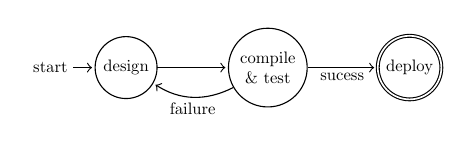
\begin{tikzpicture}[
	shorten >=1pt,
	node distance=3cm, 
	on grid, 
	auto, 
	scale=0.6, 
    transform shape, 
    align=center, 
    state/.style={
    	circle, 
    	draw, 
    	minimum size=1cm
    }] 
    
   \node[state,initial] (q_0)   {design}; 
   \node[state, right=of q_0] (q_2) {compile \\ \& test}; 
   \node[state,accepting, right=of q_2](q_3) {deploy};
   \path[->] 
    (q_0) edge node {} (q_2)
    (q_2) edge node [swap] {sucess} (q_3) 
    (q_2) edge [bend left, below] node {failure} (q_0);
\end{tikzpicture}
\caption{new development cycle}
\end{center}
\end{figure}

Protocol compiler is a tool that helps automate the process of network protocol implementation. It compiles a network protocol discriptions in a domain specific language (DSL), which declares message types and message fields, to a target programing language, like C++, Java and Python. This has saved programmer considerable amount of time by helping them to skip the implementation step, where programmers are prone to problems like nullpointer crash, sticky packet, serialization, and so on. Therefore, protocol compiler simplifies the development cycle into three simple phases (see fig~\ref{fig:newDevelopmentCycle})




\subsection{Limitation of Current Methods}

There are several protocol compilers that exists. The most commonly used one is Google's \textit{Protocol Buffers} (also known as \textit{protobuf}). Protobuf takes in a protocol declaration in their DSL called \textit{proto3} (see fig~\ref{lst:proto3}) and generates the parsing logic in a popular collection of programing languages. During the runtime, \textit{protobuf} uses BSON, the binary representation of JavaScript Object Notation (JSON), to serialize and deserialise the messages. This has given programmers the convenience to handle the data by storing the message in JSON format.\\

However, there are several drawbacks in \textit{protobuf}. These drawbakcs mainly lies in the aspect of learning curve, performance and correcness proving with formal verification.\\

First of all, although \textit{protobuf} has a well-designed DSL that concisely describes the protocol, it is one more language for the programer to learn and one more place to make mistakes. The programers need to read the documentations and do some practices in order to get started, which makes it harder to be used in fast-paced agile developent theme.\\

Moreover, when it comes to proof driven deveolpment, where, in order to prove the correctness of the implementation of the protocol, the developer needs to get the formal specification of the DSL. However, the specificaiton is not officially available, and even if it will be available in the future, it means more work for the developer, as there is one more layer of language to reason about. \\

Speaking of the performance, BSON is fairly 

\begin{figure}
\begin{center}
\lstset{language=c++}
\label{lst:proto3}
\begin{lstlisting}
message Person {
  required string name = 1;
  required int32 id = 2;
  optional string email = 3;

  enum PhoneType {
    MOBILE = 0;
    HOME = 1;
    WORK = 2;
  }

  message PhoneNumber {
    required string number = 1;
    optional PhoneType type = 2 [default = HOME];
  }

  repeated PhoneNumber phone = 4;
}
\end{lstlisting}
\caption{protocol described in proto3 language}
\end{center}
\end{figure}


\subsection{Procedureless Protocol Compiler}

\subsection{Parsly}

\section{Analysis} % Unnumbered section


\section{Conclusion} % Unnumbered section

\end{document}
